\documentclass{ltjsarticle}
\usepackage{docmute} 
\usepackage{myStyle} 

\begin{document}

\chapter{Hypothesis Testing for Factorial Designs and Differences in Means - Part 2}
\label{chapter22}
Last time, we explained that factor plans are a type of linear model, and if we view the linear model within the framework of null hypothesis testing, it corresponds to the function of the overall mean of a straight line.

In this session, we will examine both the framework of null hypothesis testing and linear models, and explore the interpretation of test results and more complex scenarios.
\section{Post Hoc Testing}
I have been explaining that hypothesis testing and linear models are just different perspectives of the same thing, but personally, I find hypothesis testing more troublesome. I feel like there are many constraints and calculations involved that make it complicated. I think it would be easier to just evaluate the magnitude of the slope while keeping the linear model, but some people might find that too formulaic. Although the calculations involved in analysis of variance may be complex, they can still be done by hand.

Now, once again, let's begin by discussing the framework of null hypothesis testing. The topic for this discussion will be analysis of variance as a combination of factor analysis and statistical judgement. More specifically, we will be comparing the null hypothesis (horizontal line model) to the alternative hypothesis (any model that isn't a horizontal line) using a model comparison approach. If you recall, for the one-factor three-level model, the alternative hypothesis corresponds to one of the following choices: \underline{which one} was it again?
\begin{itemize}
   \item Although $\mu_1 \neq \mu_2$, it is not clear whether $\mu_1=\mu_3$ or $\mu_2=\mu_3$ with regard to $\mu_3$.
   \item Although $\mu_1 \neq \mu_3$, it is not clear whether $\mu_1=\mu_2$ or $\mu_3=\mu_2$ with regard to $\mu_2$.
   \item Although $\mu_2 \neq \mu_3$, it is not clear whether $\mu_2=\mu_1$ or $\mu_3=\mu_1$ with regard to $\mu_1$.
   \item $\mu_1 \neq \mu_2 \neq \mu_3$, in other words, all are different. 
\end{itemize}

Now, as a result of the analysis of variance, a judgment has been made that it is "significant", that is to say, the null hypothesis has been rejected and the alternative hypothesis has been accepted. However, which of the alternative hypotheses is actually true is not known. This is merely a confirmation that the null hypothesis is not correct.

So, what should we do? One simple idea is to systematically test the various alternative submodels that are outlined above. For example, one could conduct an unpaired t-test between Group 1 and Group 2, between Group 1 and Group 3, and between Group 2 and Group 3. This would require three separate tests, and some people might argue that this approach could become unwieldy if there are many groups. However, with modern technology and statistical software, this process can be automated, making it a feasible and efficient option.

However, this approach does not work well as it is. The reason for this is that the null hypothesis test makes probabilistic judgments, so when it is said that there is a significant difference, there is an error (type 1 error) at the significance level $\alpha$. If this probabilistic judgment is repeated, it can actually lead to problems.

Let's consider an analogy. Suppose there is a skilled securities trader who has a good eye and can usually predict when a stock will rise in value. Of course, he occasionally makes mistakes, but let's say the chance of that happening is once every 20 times. That's a failure rate of 5%, so if a customer entrusts him with an investment, there is a 95% chance that they will make a profit. Now, on one occasion, he receives a request from a group of 10 people. Assuming he has to introduce each of them to a separate investment, can he use his 95% success rate to make all of them profitable this time?

The 5% failure rate (95% success rate) in this story is, of course, about Type 1 errors. It's the same as the risk of rejecting the null hypothesis even when it's correct (there is no difference). The fact that there are 10 requests this time is like conducting tests for each pair in a 5-level factorial design.
The possibility of making a correct judgment in one test is 95\%, but the possibility of making correct judgments two times in a row is $0.95\times0.95=0.9025$. This means that the $\alpha$ level has increased to approximately 10\%, as $1-0.9025=0.0975$! Similarly, when 10 people compete at the same time, it is $1-0.95^{10}=0.4013$, meaning there is about a 40\% chance that a mistaken judgment would be made somewhere.

Even with a 5% chance of danger and 95% accuracy, since it is a probabilistic judgment, repeating it can lead to surprisingly large numbers. Therefore, the idea that having a lot of levels means it’s fine to just repeat the t-test from the beginning is not appropriate, and repeating the t-test is not good when conducting additional tests after conducting variance analysis and determining significance.

So, what should we do from here? After this analysis of variance, we sometimes refer to the subsequent testing as \keytermE{post-hoc analysis}{かいけんてい} or \keytermE{post-hoc testing}{じごけんてい}. Many different methods are proposed for this post-hoc testing, and it is difficult to say which one is good or bad, as there are various opinions and arguments (there is even a whole book dedicated to it, \citep{BA33892274}). Nonetheless, since we can't leave it at that, let me introduce two methods here.

\paragraph{Bonferroni's method} The issue at hand is basically an inflation of the $\alpha$ level, so one possible solution is to adjust it to a lower level. For example, in this case there are three alternative hypotheses, and we want to maintain a 5% level overall, so we could judge by using $0.05/3=0.017$. This is an intuitive and easy-to-understand criterion. There are also various improved versions of this method, such as the Holm method, Shaffer's method, and Holland-Copenhaver's method.

\paragraph{Tukey's HSD Method} This is the most common and widely used method\footnote{However, "most commonly used" does not necessarily mean "correct" or "superior". Different methods have different assumptions, prerequisites, and focuses, and "most commonly used" essentially means that "statistical software packages commonly use this statistic to calculate data".} for statistical analysis. For each pair of data, a separate statistic value $q$ is calculated, and then judged whether it clears a predetermined threshold line.

In addition to these, there are various methods and options available in statistical packages. Therefore, it is important to properly record and report "which analysis method was used and how it was judged".

Above all, I want you to remember that all of these judgments are techniques used to "probabilistically" determine whether there is a difference or not. Making a determination of difference reduces a lot of data and information to just 1 bit. It is not enough to simply report that there was a difference without considering whether it was a small or significant difference. Since these judgments are also probabilistic, there is a possibility of being wrong. Depending on the method, lower-level tests may or may not be able to detect differences. Therefore, it is a misguided practice to try to find ways to create differences, which is known as p-hacking. It is more important, in terms of scientific practice, to evaluate the size of the difference and the size of the effect directly, or to consider the range of the estimated parameters.

In this section, we explained the problems of repeating hypothesis testing and their ways to avoid it. However, there is a historical context where these problems were not always emphasized even within the research practice of professional scholars. Although we gave an example of performing three tests at different levels for one analysis, the issue of "alpha inflation" would arise even if we conducted three different experiments and performed t-tests for each of them in one paper. While it is important to confirm a phenomenon by conducting multiple experiments, given that we make probabilistic judgments, we must systematically set a significant level throughout the entire process\footnote{The significant level per one analysis is called "family-wise alpha," while the significant level per one paper is called "experimental-wise alpha."}. However, in reality, researchers often repeat many t-tests for one study or fail to adjust the significant level across multiple experiments. Unfortunately, this has led to accumulated studies being "wrong." This problem can become an industry-wide crisis if each individual fails to take it seriously.

The null hypothesis test requires extremely specialized and delicate techniques to be correctly understood and used. However, because machines can easily calculate it, incorrect use of the test has become widespread. To counteract this, it is necessary to either acquire correct knowledge or stop using the null hypothesis test. There are ways to avoid making a one-bit judgment using the null hypothesis test, such as by reporting the size of confidence intervals or effect sizes. Another method is to use Bayesian estimation of probability models instead of estimation by the moment method. We may have the opportunity to talk more about the latter topic in the second half of this course.

%%%%%%%%%%%%%%%%%%%%%%% 以下，13章にて再利用
%\section{二要因の場合}
%少し話が横にそれたかもしれません。分散分析の話に戻って，今度は二要因群間計画に進んでいきたいと思います。二要因計画とはたとえば，次のような実験計画です。

%\begin{quote}
%   アサガオの生長を観察するため，水をあげる群とあげない群，肥料をあげる群とあげない群をつくり，成長の程度を比較したい
%\end{quote}

%この例では要因は「水」と「肥料」，水準はそれぞれ「あげる・あげない」なので$2\times2$の実験計画というのでした。

%アサガオの例のまま進めても良いのですが，もう少し心理学っぽいほうがイメージしやすいかもしれませんので，次のような数値例を以下では使うことにします。

%\begin{wrapfigure}{r}{6cm}
%   \centering
%    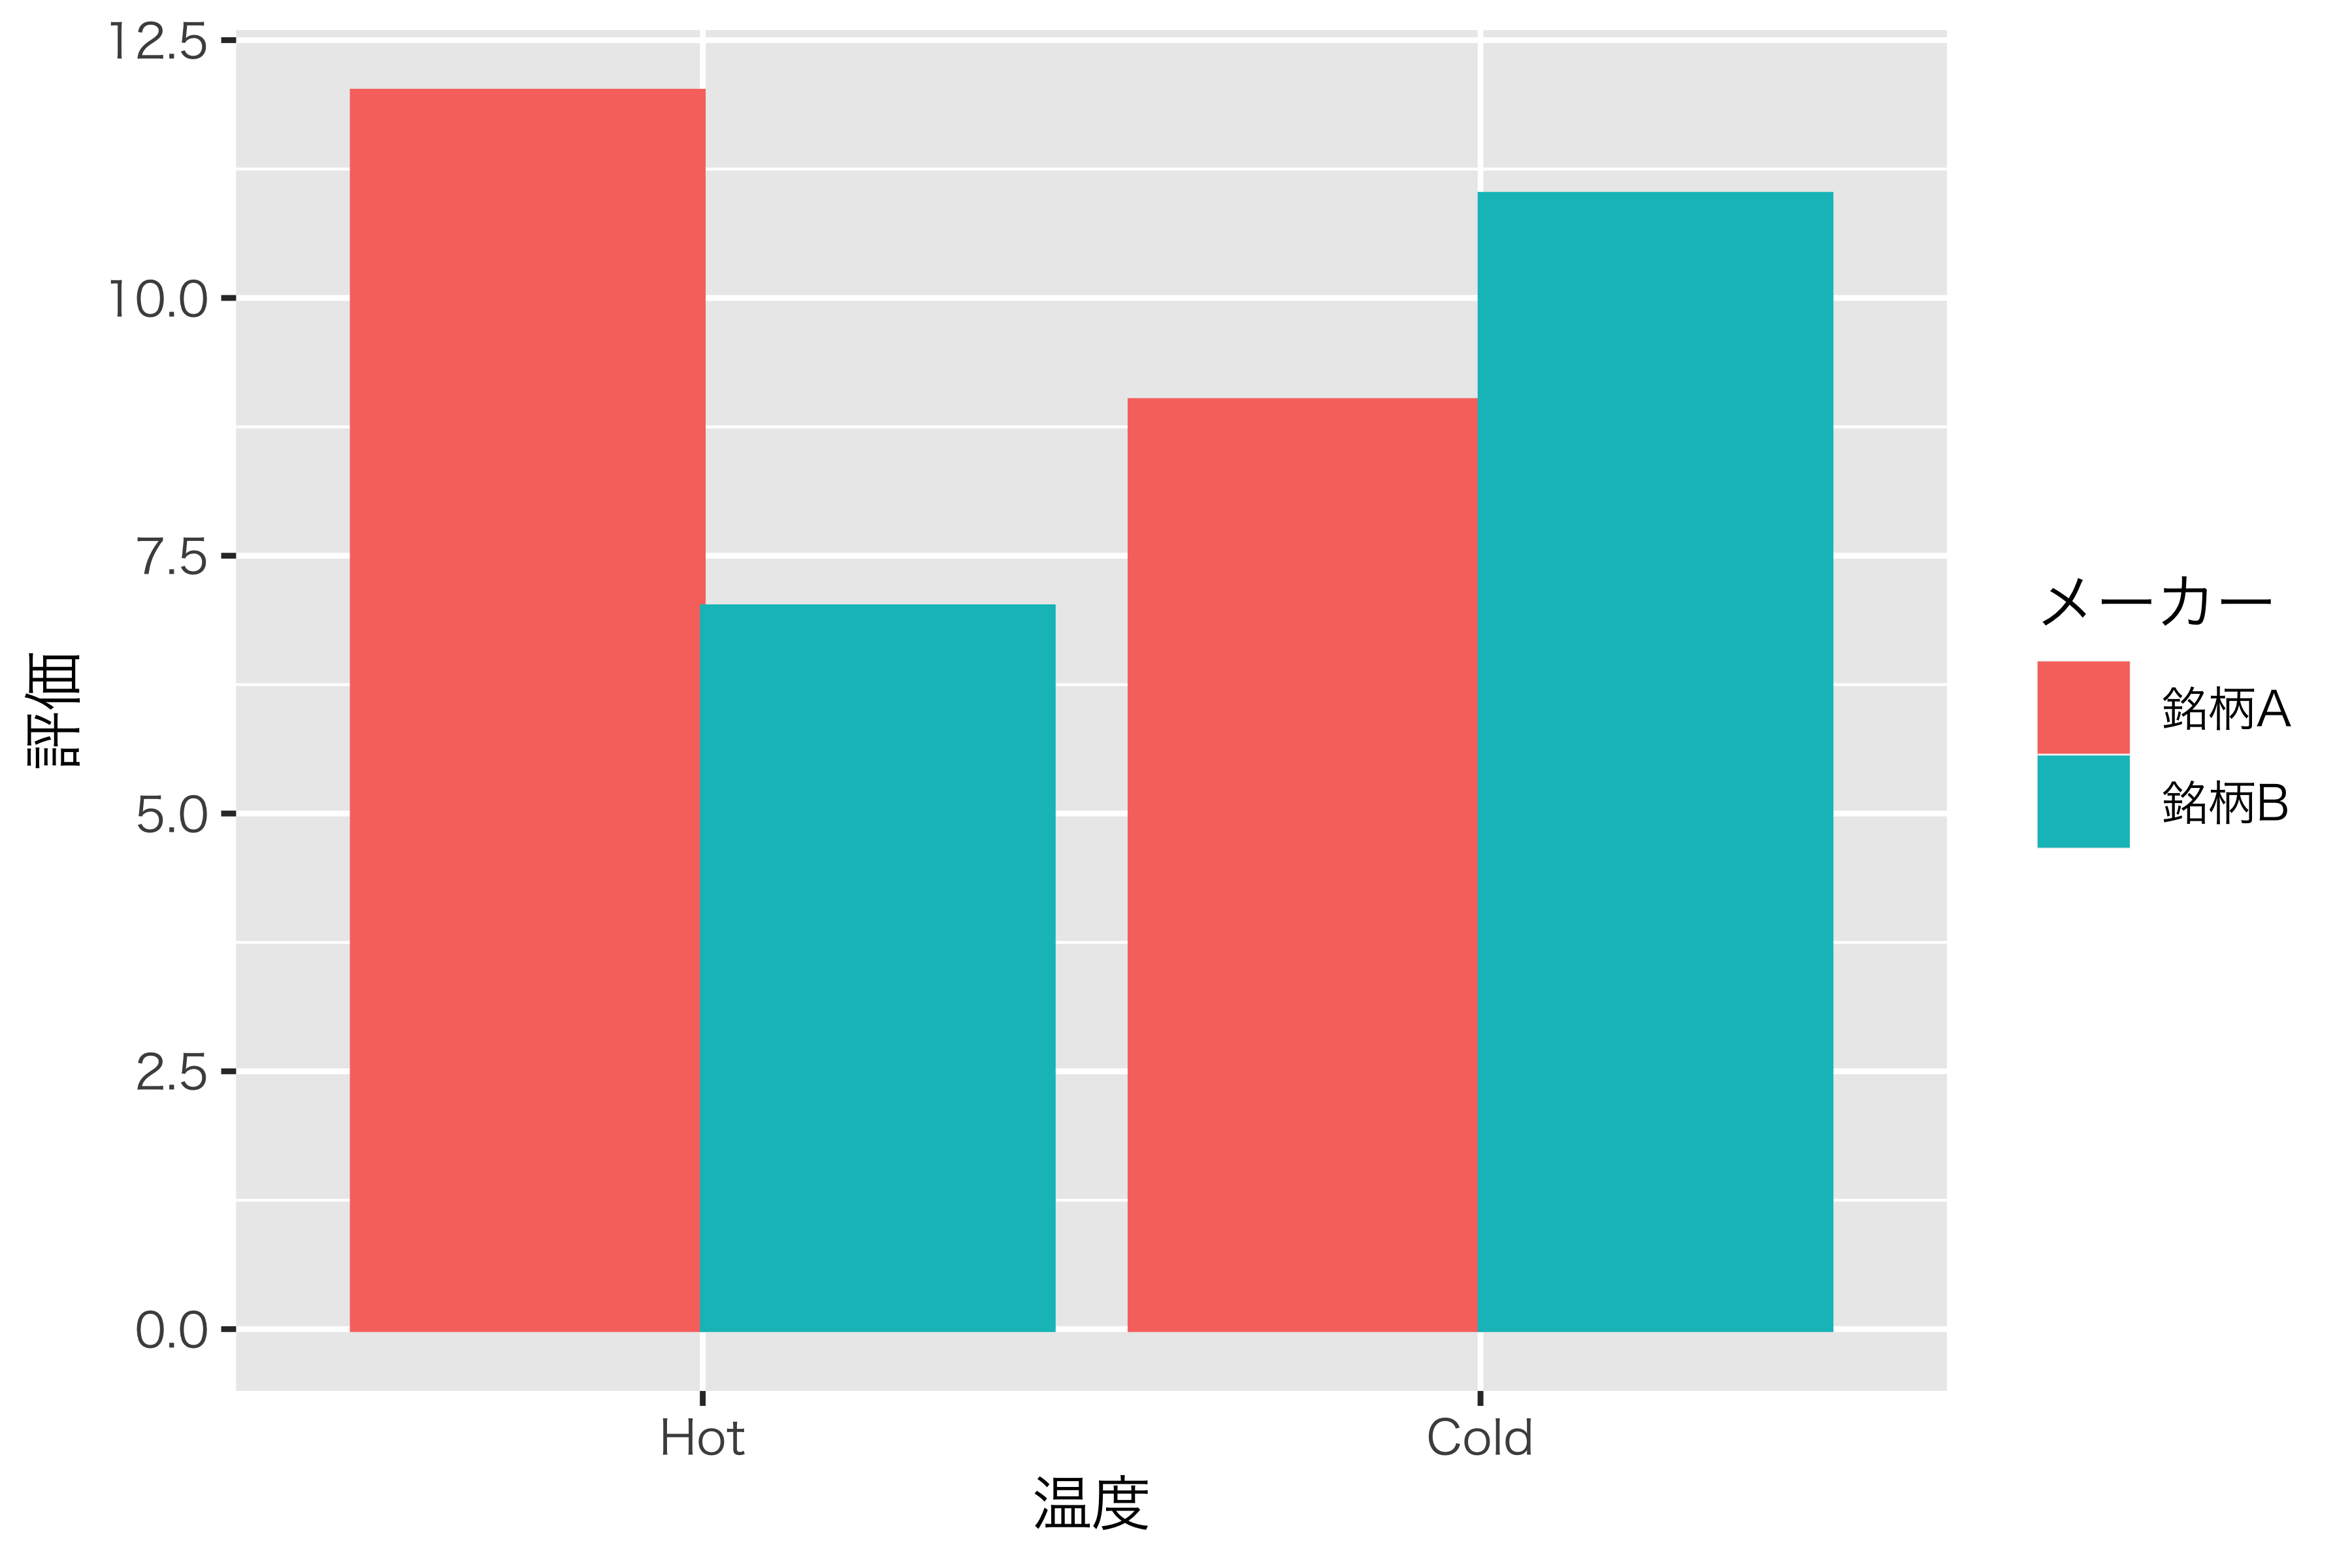
\includegraphics[keepaspectratio,width=0.5\linewidth]{../images/text22/Rplot22_01.png}
%    \caption{2種類のコーヒーと2通りの飲み方による評価}
%    \label{fig::22_01}
%\end{wrapfigure}

%2つのメーカーがそれぞれ缶コーヒーを作っていて，ホットコーヒーにした場合，アイスコーヒーにした場合の美味しさを評価してもらいます。各条件に3名ずつ試飲をお願いして，20点満点で評価してもらったら，表\ref{tbl::22_01}のようになりました。これを図示したのが図\ref{fig::22_01}にあります。これを見るとわかるように，ホットコーヒーにすると銘柄Aは高い評価，アイスコーヒーだと両者の違いはなくなることがわかります。どうも銘柄Bはホットコーヒーにして売らない方がいいように思いますが，とはいえこれらも標本平均のはなしであって，たまたまホットの銘柄Bを飲んだ3人がコーヒーが苦手だったのかもしれない。標本平均ではなく母平均で話をするために，このデータについて考えていきたいと思います。
% latex table generated in R 4.0.2 by xtable 1.8-4 package
% Fri Sep 11 14:11:29 2020
%\begin{table}[ht]
%  \centering
%  \caption{二要因のデータ例} 
%  \begin{tabular}{rrllr}
%    \hline
%  通し番号 & 群での番号 & 温度 & メーカー & 評価 \\ 
%    \hline
%  1 & 1 & Hot & 銘柄A & 13 \\ 
%    2 & 2 & Hot & 銘柄A & 11 \\ 
%    3 & 3 & Hot & 銘柄A & 12 \\ 
%    4 & 1 & Hot & 銘柄B & 7 \\ 
%    5 & 2 & Hot & 銘柄B & 6 \\ 
%    6 & 3 & Hot & 銘柄B & 8 \\ 
%    7 & 1 & Cold & 銘柄A & 9 \\ 
%    8 & 2 & Cold & 銘柄A & 9 \\ 
%    9 & 3 & Cold & 銘柄A & 9 \\ 
%    10 & 1 & Cold & 銘柄B & 13 \\ 
%    11 & 2 & Cold & 銘柄B & 11 \\ 
%    12 & 3 & Cold & 銘柄B & 9 \\ 
%     \hline
%  \end{tabular}

%  \label{tbl::22_01}
%  \end{table}


%\subsection{線形モデルとしてみた二要因計画}
%一要因の計画も，線形モデルと見ることができるという話をしました。二要因の計画も当然，同じように線形モデルとして考えることができます。

If we were to express the Ishikawa diagram as a linear model,
%\[ X_{ij} = \beta_0 + \beta_1 X_j + \varepsilon_{ij} \]
%と書くことができるのでした。ここで$X_j$は前回，プラスとマイナスの符号を表すためだけに用意したもので，一方が実験群，他方が統制群を表している，という名義尺度水準の数値でしたね。

%さて今回は二要因計画です。要因は「温度」と「メーカー」の二種類ありますから，効果として$\beta_1$と$\beta_2$の2つが必要です。これを式に書き入れてみますと，
%\begin{equation}
%    \label{eq22_01}
%X_{ijk} = \beta_0 + \beta_1 X_j + \beta_2 X_k + \varepsilon_{ijk}
%\end{equation}
%のようにかけるでしょう。ここで$X_{ijk}$と3つも添字がついていますが，表\ref{tbl::22_01}にあるように，$i$は群での個人を特定する番号，$j$は温度がHot/Coldのどちらに割り当てられたか，$k$は銘柄A/Bどちらに割り当てられたか，を意味しています。$X_j$はHotなら$+1$，Coldなら$-1$で，$X_k$は銘柄Aなら$+1$，銘柄Bなら$-1$になります。これは温度やメーカーの効果は全体平均からみて相対的にプラスなのか，マイナスなのかを表しているからです。図\ref{fig::22_02}に，群ごとに平均値をプロットし，全体平均(9.75)のラインを横一線で引いてみました。これを見ると，各群の効果が全体平均を挟んで，相対的に同じ大きさで出ているのがわかると思います。
%\begin{figure}[ht]
%    \centering
%    
\includegraphics[keepaspectratio,width=0.8\linewidth]{../images/text22/Rplot22_02.png}
%    \caption{群ごとにプロットしたもの。全体平均から見た相対評価になっていることが確認できる。}
%    \label{fig::22_02}
%\end{figure}

%さて改めて式\ref{eq22_01}を見ると，これも線形モデル，とくに説明変数が複数ある重回帰分析のモデルと同じ形をしているのが分かりますね。重回帰分析は第\ref{chapter9}でやりましたが，そのモデル式は
%\[ y_i = b_0 + b_1 x_{1i} + b_2 x_{2i} +e_i \]
%であり，$b$と$\beta$の違いはありますが，基本的に同じ形をしているのが確認できると思います。要因計画は線形モデルなのです。

%\paragraph{効果と誤差の析出}
%さてそれでは，効果の大きさ，誤差の大きさを見積もってみましょう。二要因の場合でも考え方は同じです。基本的に同じ母平均を持っているところから出てきた標本で，何の手も加えなければ，評定値の違いも生じないのですが，やれ温度の操作だとか，やれメーカーの違いだとかで人によって違う介入があり，しかも人間のやることですので個人差も加わってしまう。だから見た目のデータがばらついているんだ，と考えるのです。

%理想的には全部同じはず，つまり母平均に違いがないという帰無仮説の世界を考えると，得られるデータは全体平均$\bar{X}_{gm} = 9.75$にぴったり合致するはずなのでした。しかしそこに温度の効果$\beta_1$が関係してきます。図\ref{fig::22_02}の左にあるように，温度で群わけをするとHot群だけの平均は
%\[ \frac{1}{6} (13+11+12+7+6+8)= 9.5 \]
%で，Cold群だけの平均は
%\[ \frac{1}{6}(9+9+9+13+11+9) = 10.0 \]
%になります。全体平均から考えると，Hot群に割り当てられると$-0.25$の効果が，Cold群に割り当てられると$+0.25$の効果があったようです($\beta_1$の推定値)。

%同様に，メーカーの効果も考えましょう。銘柄Aの平均値は，
%\[ \frac{1}{6}(13+11+12+9+9+9) = 10.5 \]
%ですし，銘柄Bの平均値は
%\[ \frac{1}{6}(7+6+8+13+11+9)= 9.0 \]
%ですから，銘柄Aは全体平均より$10.5-9.75=0.75$高くなる効果が，相対的に銘柄Bは全体平均より$0.75$下がる効果がある，ということがわかります。

%さて，これらの効果がわかったところで，足し算を組み上げていきましょう。全体平均にそれぞれの効果を加えていきます。銘柄Aをホットコーヒーでいただくとすると，全体平均$ 9.75$にホット($-0.25$)の銘柄A($+0.75$)ですから，$9.75-0.25+0.75=10.25$となり，これが銘柄Aをホットで飲んだ時の平均値に・・・

%なりませんでした($\frac{1}{3}(13+11+12)=12$)。あれ? 
%\paragraph{ただしイケメンに限る}
%同様のことは他の組み合わせのところでも生じます。群平均からの差分が誤差なのだ，と考えれば良いのですが，群平均が理論通りになりません(表\ref{tbl::22_02}に計算してみました。効果の総和と群平均，理論的には合致するはずです)。これはどうしたことでしょう。
%\begin{table}[ht]
%    \centering
%    \caption{二要因のデータ例} 
%    \begin{tabular}{rrrccr}
%      \hline
%    全体平均 & 温度の効果 & メーカーの効果 & 効果を足し合わせると & 群平均は & 評価 \\ 
%      \hline
%    9.75 & -0.25 & +0.75 & \multirow{3}{*} {10.25} & \multirow{3}{*}{12.0} & 13 \\ 
%    9.75 & -0.25 & +0.75 & & & 11 \\ 
%    9.75 & -0.25 & +0.75 & & & 12 \\ \hline
%    9.75 & -0.25 & -0.75 & \multirow{3}{*} {8.75} & \multirow{3}{*}{7.0} & 7 \\ 
%    9.75 & -0.25 & -0.75 & & & 6 \\ 
%    9.75 & -0.25 & -0.75 &  & & 8 \\ \hline
%    9.75 & +0.25 & +0.75 & \multirow{3}{*} {10.75} & \multirow{3}{*}{9.0} & 9 \\ 
%    9.75 & +0.25 & +0.75 & & & 9 \\ 
%    9.75 & +0.25 & +0.75 & & & 9 \\ \hline
%    9.75 & +0.25 & -0.75 & \multirow{3}{*} {9.25} & \multirow{3}{*}{11.0} & 13 \\ 
%    9.75 & +0.25 & -0.75 & & & 11 \\ 
%    9.75 & +0.25 & -0.75 & & & 9 \\ 
%       \hline
%    \end{tabular}
%    \label{tbl::22_02}
%\end{table}
%銘柄A($+0.75$)のホットコーヒー($-0.25$)が10.25で，群平均が12.0ということは，$12.0-10.25=+1.75$の効果が出ていることになります。これは「Aをホットで」という組み合わせの時にのみ生じる組み合わせの効果で，とくに\keytermE{交互作用}{こうごさよう}{interaction}といいます\footnote{余談ですが，統計的な文脈ではinteractionを「交互作用」と訳します。社会心理学などの文脈では，「相互作用」と訳されます。}。交互作用とはこのように，水準同士の組み合わせによって生じる特別な効果のことを指します。交互作用に対して，これまでみてきた群の平均は\keytermE{主効果}{しゅこうか}{main effect}と呼んで区別します。式\ref{eq22_01}にあった線形モデルは，次の式\ref{eq22_02}のように交互作用項も含めたものにアップデートしなければなりません。
%\begin{equation}
%  \label{eq22_02}
%X_{ijk} = \beta_0  + \beta_1 X_j  + \beta_2 X_k + \beta_3 X_{jk} + \varepsilon_{ijk}
%\end{equation}

%この交互作用は，式\ref{eq22_02}にもあるように，主効果とは別の独立した影響源です。ですから，主効果がなくても，交互作用だけある，ということがあり得ます。このパラグラフのタイトルにもあるように，交互作用はいわば「ただしイケメンに限る」という条件のようなものです。かっこいいセリフや仕草は，それぞれに評価を上げる効果がなくとも(あってもいいんですが)，イケメンがするからとくに良いのであって，イケメンでない人がするとむしろ逆効果，ということもあるのでそれを考慮しておこう，ということです\footnote{このたとえはポリコレ的に正しくないというか，恋愛至上主義的で容姿に基づく人物評価を助長するような笑いの形式になっているので，個人的には好ましく思っていないのです。が，みなさんが交互作用を身近に感じてもらえるのでは，と思って書いています。個人的には熱燗で飲む日本酒と冷やで飲む日本酒って違うよね，という例のが一番ピンとくるんですが，お酒を飲まない人，あるいは未成年の方にとってはこれも不適切な例かなと思ったり。本文はコーヒーにしていますが，わかりやすい例になっているでしょうか。何か良いアイデア，たとえがありましたら，ご一報ください。}。

%さて，この組み合わせの効果も相対的なもので，全部足し合わせると$0$になります。全体としては効果$0$であり，こちらで人為的に区切ることによって差分が生じている，と考えているからです。実際これを見ると，銘柄A($+0.75$)のアイスコーヒー($-0.25$)の効果が全体平均に加わると$8.75$で，群平均が$7.0$ですから，ここには$-1.75$の交互作用効果が出ています。同様に銘柄Bのホットには$-1.75$，銘柄Bのアイスには$+1.75$ですから，4つの要素を足すとキャンセルしあって合計$0$ですね。

%交互作用のもつ符号は，プラスとマイナスが上から順に$+,-,-,+$となっています。どうしてこういうことになっているのかについて，説明を追加しておきましょう。
%今回は$2\times2$の計画ですから，図\ref{fig::22_01}にあるように組み合わせの表を書いてみると，主効果はその周辺の平均値で考えていたことがわかります。たとえば1つ目の要因である温度(図中では要因Aとします)の，「ホット(水準a1)」か「アイス(水準b1)」かの話は，もう1つの要因であるメーカーを潰して，列方向に1つのグループにした平均からその効果を計算していました($\beta_1$)。この水準同士の比較は相対的なので，水準1と2は符号違いで$+\beta_1,-\beta_1$になっています。同様に，2つ目の要因であるメーカー(図中では要因Bとします)についても，要因Aの水準を潰して行方向に1つのグループと考え，平均を出して効果を算出し，相対比較にしていました($+\beta_2,-\beta_2$)。

%これに対して，交互作用はセル内，各組み合わせについて生じている効果です。行方向，列方向についてはそれぞれの要因の主効果として計算されていますから，交互作用は行方向に足し合わせてもプラマイ0，列方向に足しあわせてもプラマイ0になる必要があります。そうでないと，主効果が変わってきてしまうからです。図\ref{fig::22_04}の左上，a1b1水準に交互作用効果$\beta_3$が生じたとすると，列方向，つまり同じ水準a1のなかで，総和がゼロにならないといけませんから，a1b2水準には$-\beta_3$が入ることになります。これはまた，行方向にも総和がゼロ出なければなりませんから，a2b1も$-\beta_3$である必要があります。残る右下のa2b2は，行方向にも列方向にも総和ゼロにするためには$+\beta_3$でなければなりません。このようにして，交互作用の符号は周りとの関係で定まっていたのです。交互作用の大きさは，どの行方向，列方向をみても総和ゼロになっている，というのは水準数が増えても同じです。

%\begin{figure}[ht]
%  \begin{tabular}{cc}
%---- 最初の図 ---------------------------
%    \begin{minipage}[t]{0.45\hsize}
%      \centering
%      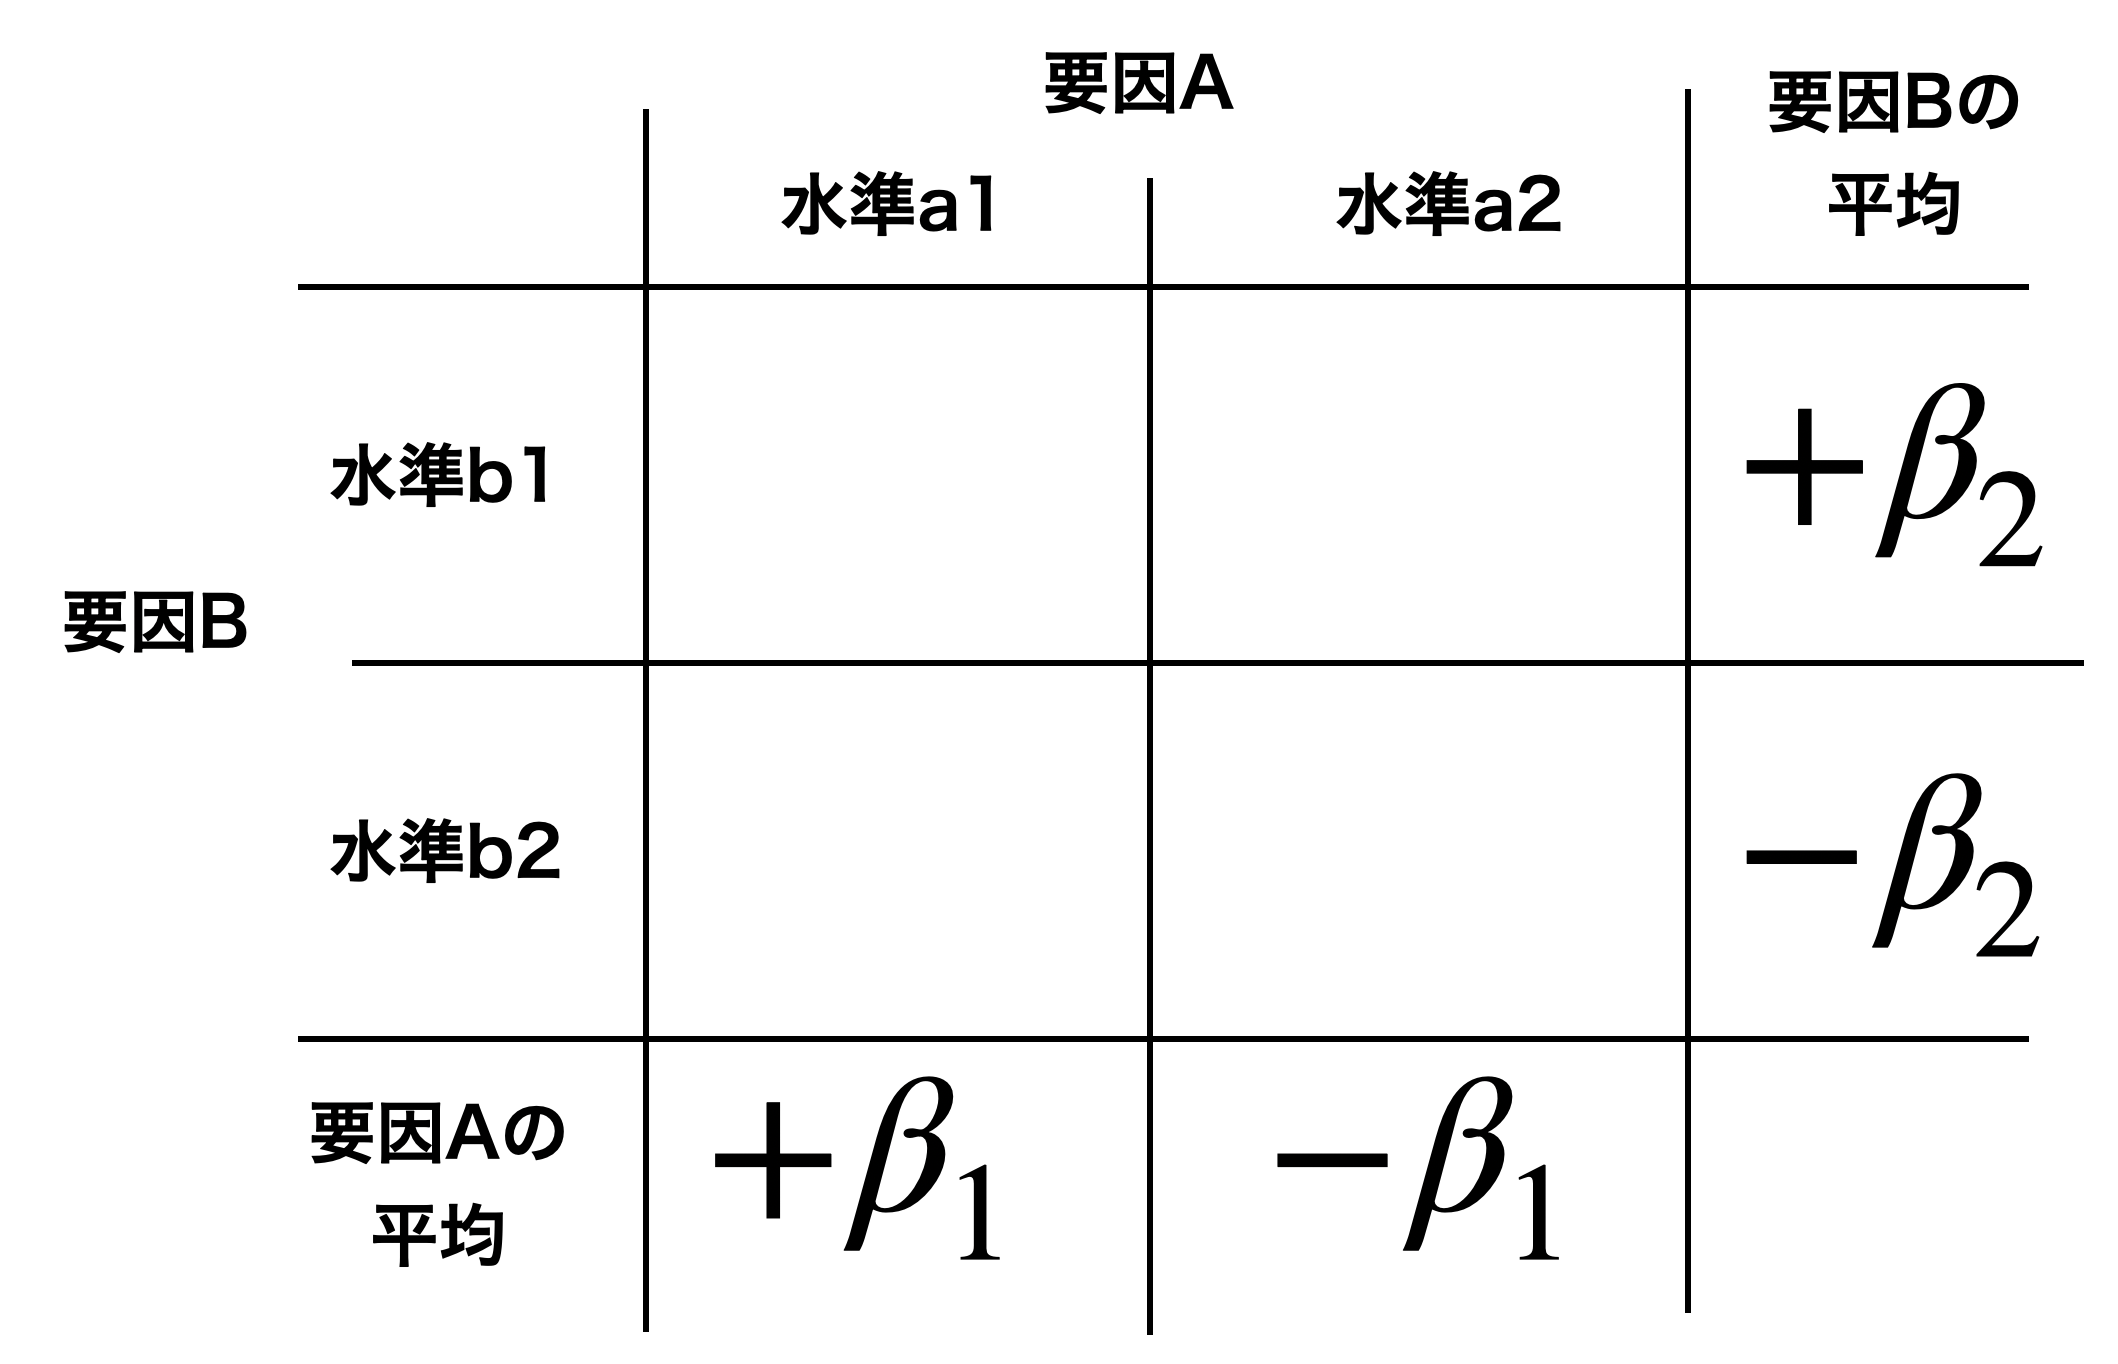
\includegraphics[keepaspectratio,width=0.5\linewidth]{../images/text22/slide22_01.png}
%      \caption{主効果の計算は周辺の平均値から計算する}
%      \label{fig::22_03}
%    \end{minipage} &
%    %---- 2番目の図 --------------------------
%    \begin{minipage}[t]{0.45\hsize}
%      \centering
%      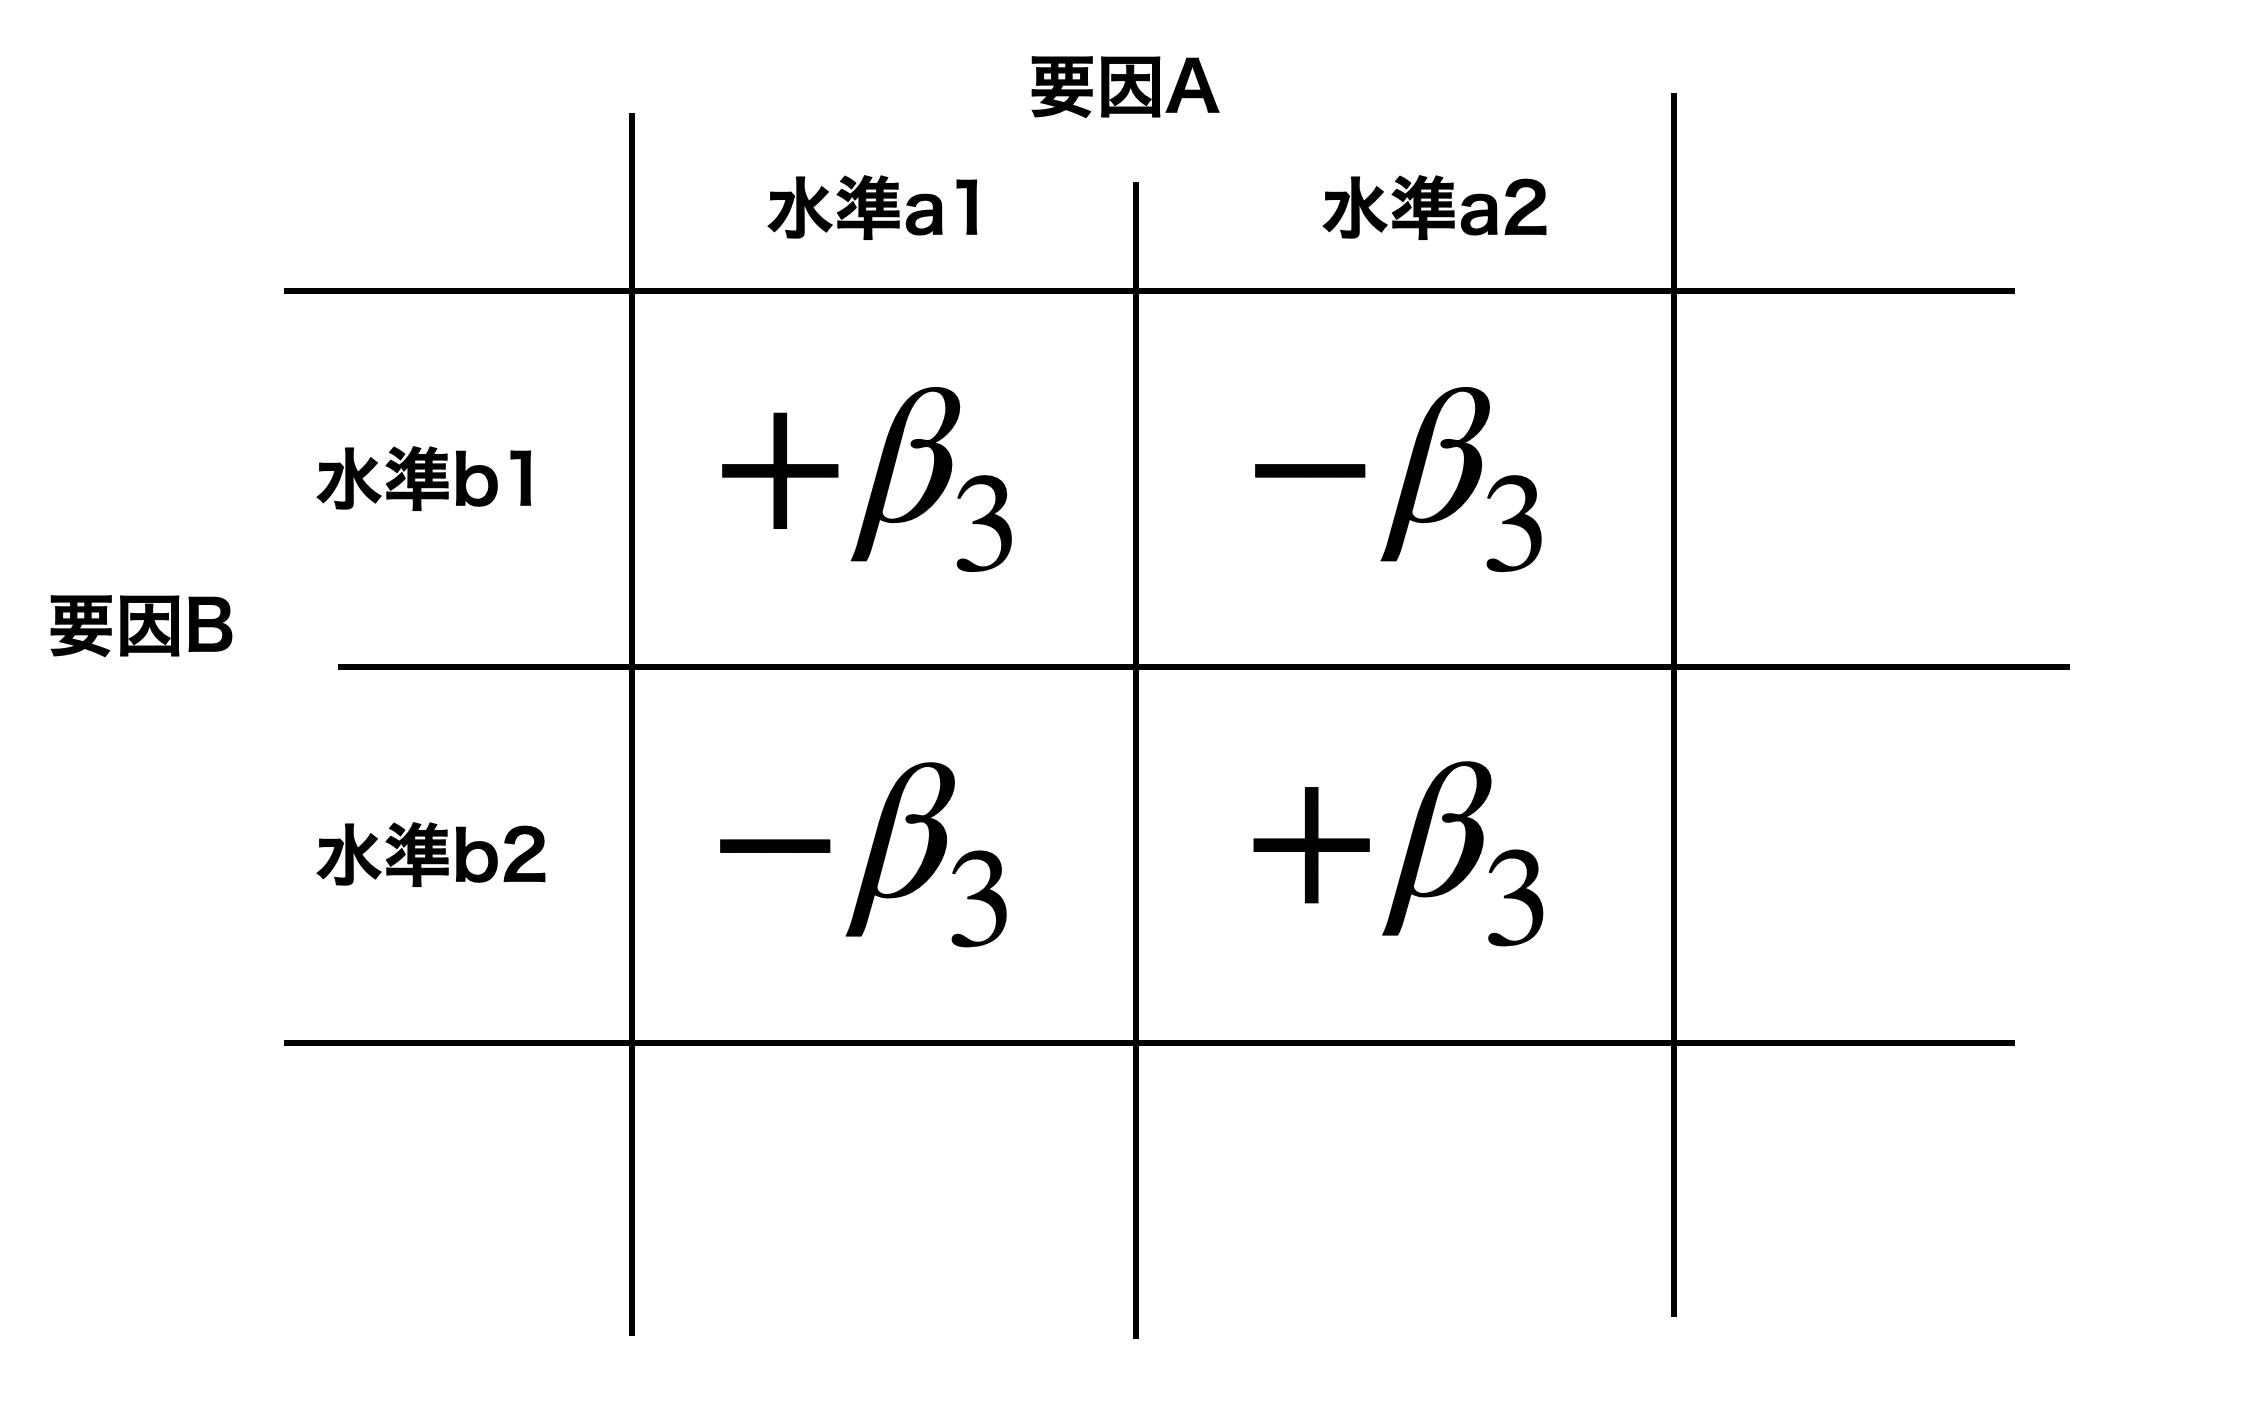
\includegraphics[keepaspectratio,width=0.5\linewidth]{../images/text22/slide22_02.png}
%      \caption{交互作用はセルの内部で相殺するように}
%      \label{fig::22_04}
%    \end{minipage}
%    %---- 図はここまで ----------------------
%  \end{tabular}
%\end{figure}%
%このように交互作用を含めて計算すると，組み合わせ水準のところまではしっかりと計算が合うようになります。それでも一人ひとりのレベルまで含めて考えてみると，やはりズレが出てしまいますが，これはどうしようもない個人差＝誤差ですので，これを計算することで誤差を算出できます。

%\begin{table}[ht]
%  \centering
%  \caption{平方和の計算} 
%  \begin{tabular}{rrrccr}
%    \hline
% 全体平均 & 温度の効果 & メーカーの効果 & 交互作用 & 誤差 & 評価 \\ 
%    \hline
%  9.75 & -0.25 & +0.75 &  +1.75 & +1.00 & 13 \\ 
%  9.75 & -0.25 & +0.75 & +1.75& -1.00 & 11 \\ 
%  9.75 & -0.25 & +0.75 & +1.75& 0.00 & 12 \\ \hline
%  9.75 & -0.25 & -0.75 &-1.75 & 0.00 & 7 \\ 
%  9.75 & -0.25 & -0.75 & -1.75& -1.00& 6\\ 
%  9.75 & -0.25 & -0.75 & -1.75 & +1.00& 8 \\ \hline
%  9.75 & +0.25 & +0.75 & -1.75 & 0.00 & 9 \\ 
%  9.75 & +0.25 & +0.75 & -1.75& 0.00& 9 \\ 
%  9.75 & +0.25 & +0.75 & -1.75 & 0.00& 9 \\ \hline
%  9.75 & +0.25 & -0.75 & +1.75 & +2.00 & 13 \\ 
%  9.75 & +0.25 & -0.75 & +1.75 & 0.00& 11 \\ 
%  9.75 & +0.25 & -0.75 & +1.75 & -2.00& 9 \\ 
%     \hline\hline
%平方和 & 0.75 & 6.75 & 36.75 & 12.00 & \\\hline
%  \end{tabular}
%  \label{tbl::22_03}
%\end{table}
%表\ref{tbl::22_03}には，それぞれの効果の大きさと平方和を計算したものを書きました。二乗して足し合わせたのはもちろん，大きさを比較して判定に持ち込むためです。
\section{Two-Factor Linear Model as a Test of Null Hypothesis}
Analysis of variance is an approach to testing for differences in means across multiple levels. When there are more than two factors, it is guaranteed to have at least three levels, necessitating the use of analysis of variance. Following the formal procedures of the null hypothesis test, we can consider the following:
\paragraph{Setting the hypothesis} Both the null hypothesis and the alternative hypothesis are required. As previously mentioned, the null hypothesis is that there is no difference in the population mean. In this case, it means that no matter where you cut it, there is no difference in the population mean. If we take the first level of the first factor (the "Hot" temperature factor) and the second level of the second factor (the "Brand B" manufacturer factor) and denote their population mean as $\mu_{12}$, then the null hypothesis can be stated as $H_0:\mu_{11}=\mu_{12}=\mu_{21}=\mu_{22}$. The alternative hypothesis is the negation of the null hypothesis.
\paragraph{Select Test Statistic} Although we are estimating the mean value, since we are testing the variance, we will use a tool called $F$ distribution.
\paragraph{Setting the criteria for judging probability} Let's set the significance level at $\alpha$, and again, let's make the decision with a 5\% probability.
\paragraph{Calculating the realized value of the test statistic} The realized value of the test statistic $F$ is calculated based on the sums of squares presented in table \ref{tbl::22_03}. After accounting for degrees of freedom and adjusting for the magnitude of the effect per unit, comparisons can be made. Therefore, let's summarize and display the results in an ANOVA table.
% latex table generated in R 4.0.2 by xtable 1.8-4 package
% Fri Sep 11 14:39:12 2020
\begin{table}[ht]
   \centering
   \caption{ANOVA Table}
   \begin{tabular}{lrrrrr}
      \hline
           & Df    & SS     & MS     & F value & $p$   \\
      \hline
      Temperature   & 1.000 & 0.750  & 0.750  & 0.500   & 0.500 \\
      Manufacturer & 1.000 & 6.750  & 6.750  & 4.500   & 0.067 \\
      Interaction & 1.000 & 36.750 & 36.750 & 24.500  & 0.001 \\
      Error   & 8.000 & 12.000 & 1.500  &         &       \\
      \hline
   \end{tabular}
   \label{tbl::22_04}
\end{table}

Looking at this, we can see that there is no main effect for temperature ($F(1,8)=0.50,p=0.500$) or for manufacturer ($F(1,8)=4.50,p=0.067$), but there is an interaction effect ($F(1,8)=24.50,p=0.001$). Since there are two levels for each factor in this case, we do not need to conduct any post-hoc tests for the main effects. However, if an interaction effect is present, further analysis is needed to determine where the differences lie. Data is divided for each level (the first and second level of factor A, and the first and second level of factor B), and then an exploration is conducted to determine where the differences lie. In this example, we would need to investigate the following four patterns: 1. Is there a difference between brand A/B when the temperature is hot? 2. Is there a difference between brand A/B when the temperature is cold? 3. Is there a difference between hot and cold for brand A? 4. Is there a difference between hot and cold for brand B? Of course, there is an issue with multiple tests, so we would need to correct for this using methods such as Bonferroni or Tukey.

In addition, it would be good to calculate and report the effect size. These details are often automatically generated by statistical packages, so we will leave them for when we cover R in our exercises.

% \section{Within計画の場合}
% 線形モデルと帰無仮説検定「講義編」，最後の山場は群内計画・反復測定・Withinデザインの場合です。
% 今回も数値例を基に話を始め，線形モデルでの表現と帰無仮説検定での判定，という二段階で進めて行きたいと思います。

% 今回は一要因3水準の，群内計画の要因計画の話をしましょう。データに対応がある，あるいは反復測定であることがポイントです。同じ人に複数回データを提供してもらう，次のような状況をイメージしてください。

% 臨床心理学者がある介入法をつかってメンタルケアに取り組んでいます。4人のクライアントにこの手法を適用し，抑うつ度が改善されていくかどうかチェックします。表\ref{tbl::22_05}のようなスコアが得られたとき，この介入法に効果あるかどうかを考えたい，とします。
% % latex table generated in R 4.0.2 by xtable 1.8-4 package
% % Fri Sep 11 14:57:29 2020
% \begin{table}[ht]
%   \centering
%   \caption{Within Data Example} 
%   \begin{tabular}{lrrr}
%     \hline
%   ID & Time1 & Time2 & Time3 \\ 
%     \hline
%   1 & 10 & 5 & 9 \\ 
%     2 & 9 & 4 & 5 \\ 
%     3 & 4 & 2 & 3 \\ 
%     4 & 7 & 3 & 5 \\ 
%      \hline
%   \end{tabular}
%   \label{tbl::22_05}
%   \end{table}
% このデータを図にしてみましょう。ポイントは，3つの調査時点(Time1,2,3)それぞれが独立ではなく，クライアント番号(ID)は共通しているというところです。横軸は時間だとすると，その軸に意味がありますから，同じ人のデータ点を線で結ぶことができるのです。

% \begin{wrapfigure}{r}{8cm}
%   \centering
%   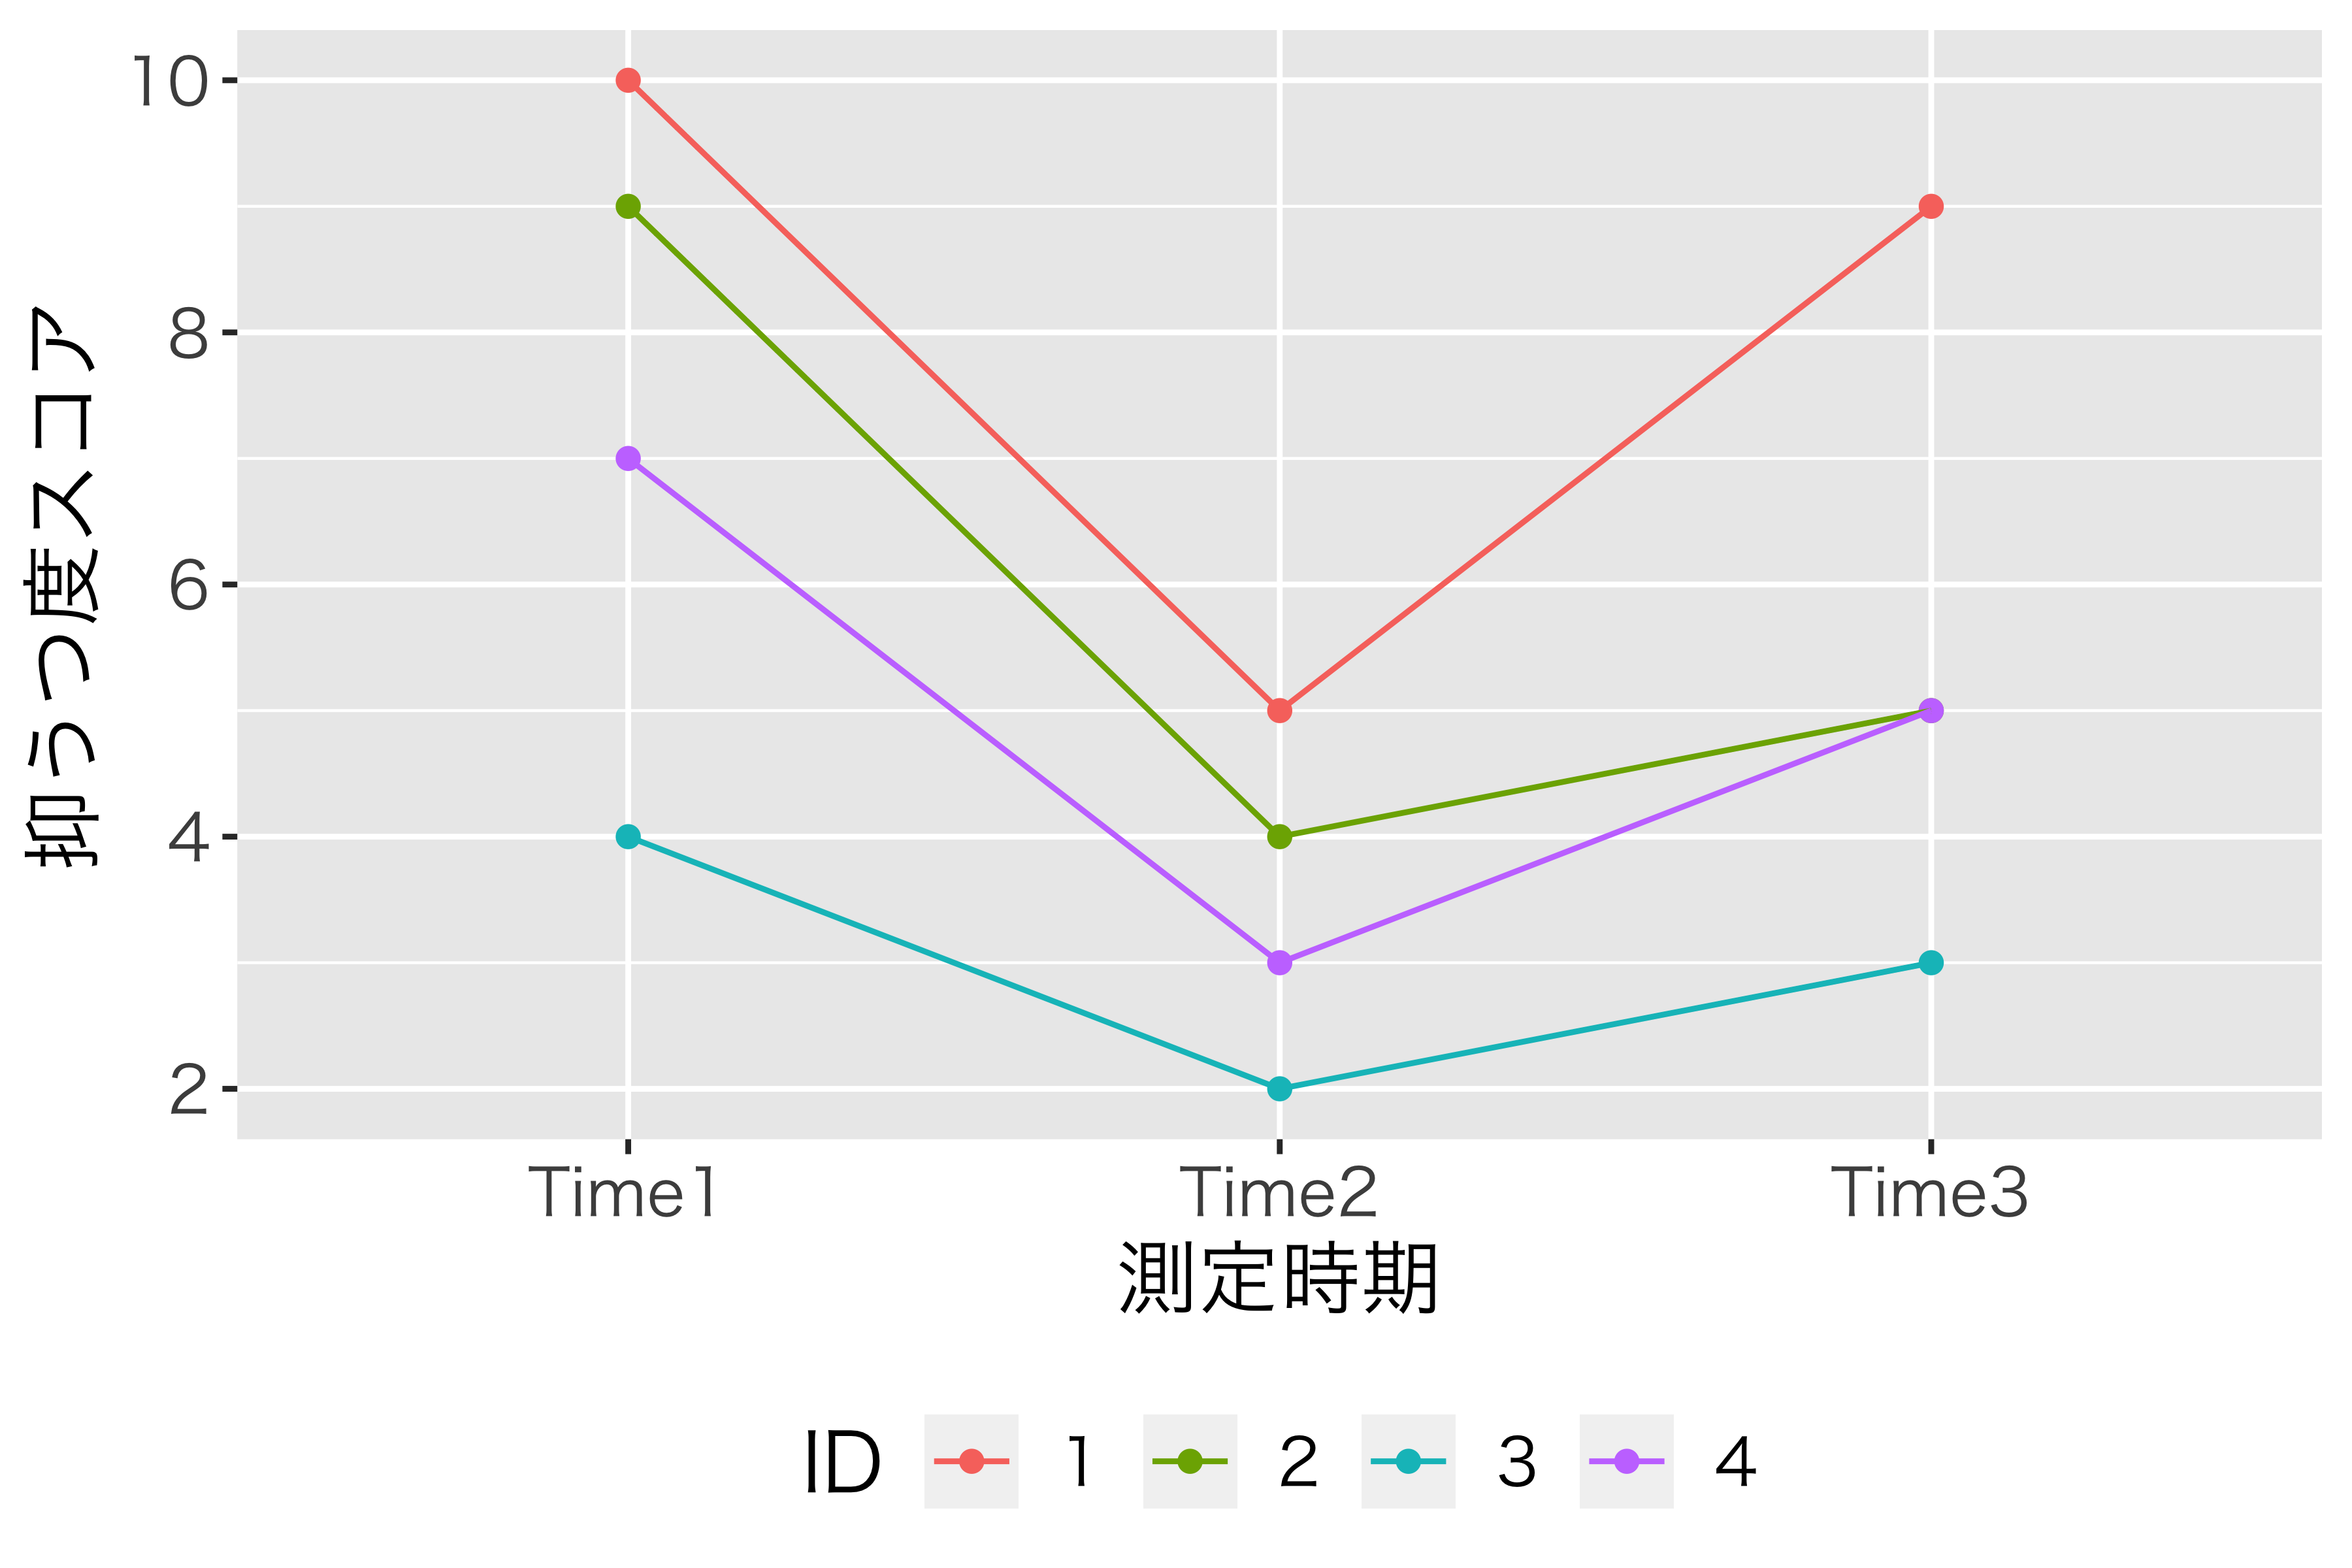
\includegraphics[keepaspectratio,width=0.65\linewidth]{../images/text22/Rplot22_03.png}
%   \caption{介入効果によるクライアントの状態変化}
%   \label{fig::22_05}
% \end{wrapfigure}
% 図\ref{fig::22_05}をみていると，個人差こそあれ，第一期(Time1)から二期(Time2)にかけてはいったん下降傾向があり，第二期から三期(Time3)にかけては上昇傾向があるのかなあ，と思ったりします。この直感をデータで検証してくことが大事ですね。

% ここで考えたいのは，「個人差こそあれ」のところです。個人差があるというのは，最初10点から始まるのか(ID=1)，4点から始まるのか(ID=3)，というところで既に7点差ついてるのですが，今回これは個人差であってみたい効果の部分ではない，と考えるということです。見たい効果は「時期」要因による，3つの水準それぞれへの影響，$\beta_{1j}$ なのです。数式的に表現すると，個人$i$ の第$j$期におけるデータ$X_{ij}$は，
% \[ X_{ij} = \mu_i + \beta_0 + \beta_{ij} + \varepsilon_{ijk} \]
% となります。ポイントとして，新たに$\mu_i$というのが出てきました。これは$i$に伴って変わる数字で，時期$j$の添字がついていませんから，「時期を通して一貫した個人の平均値」ということになります。
% \begin{figure}[ht]
%   \centering
%   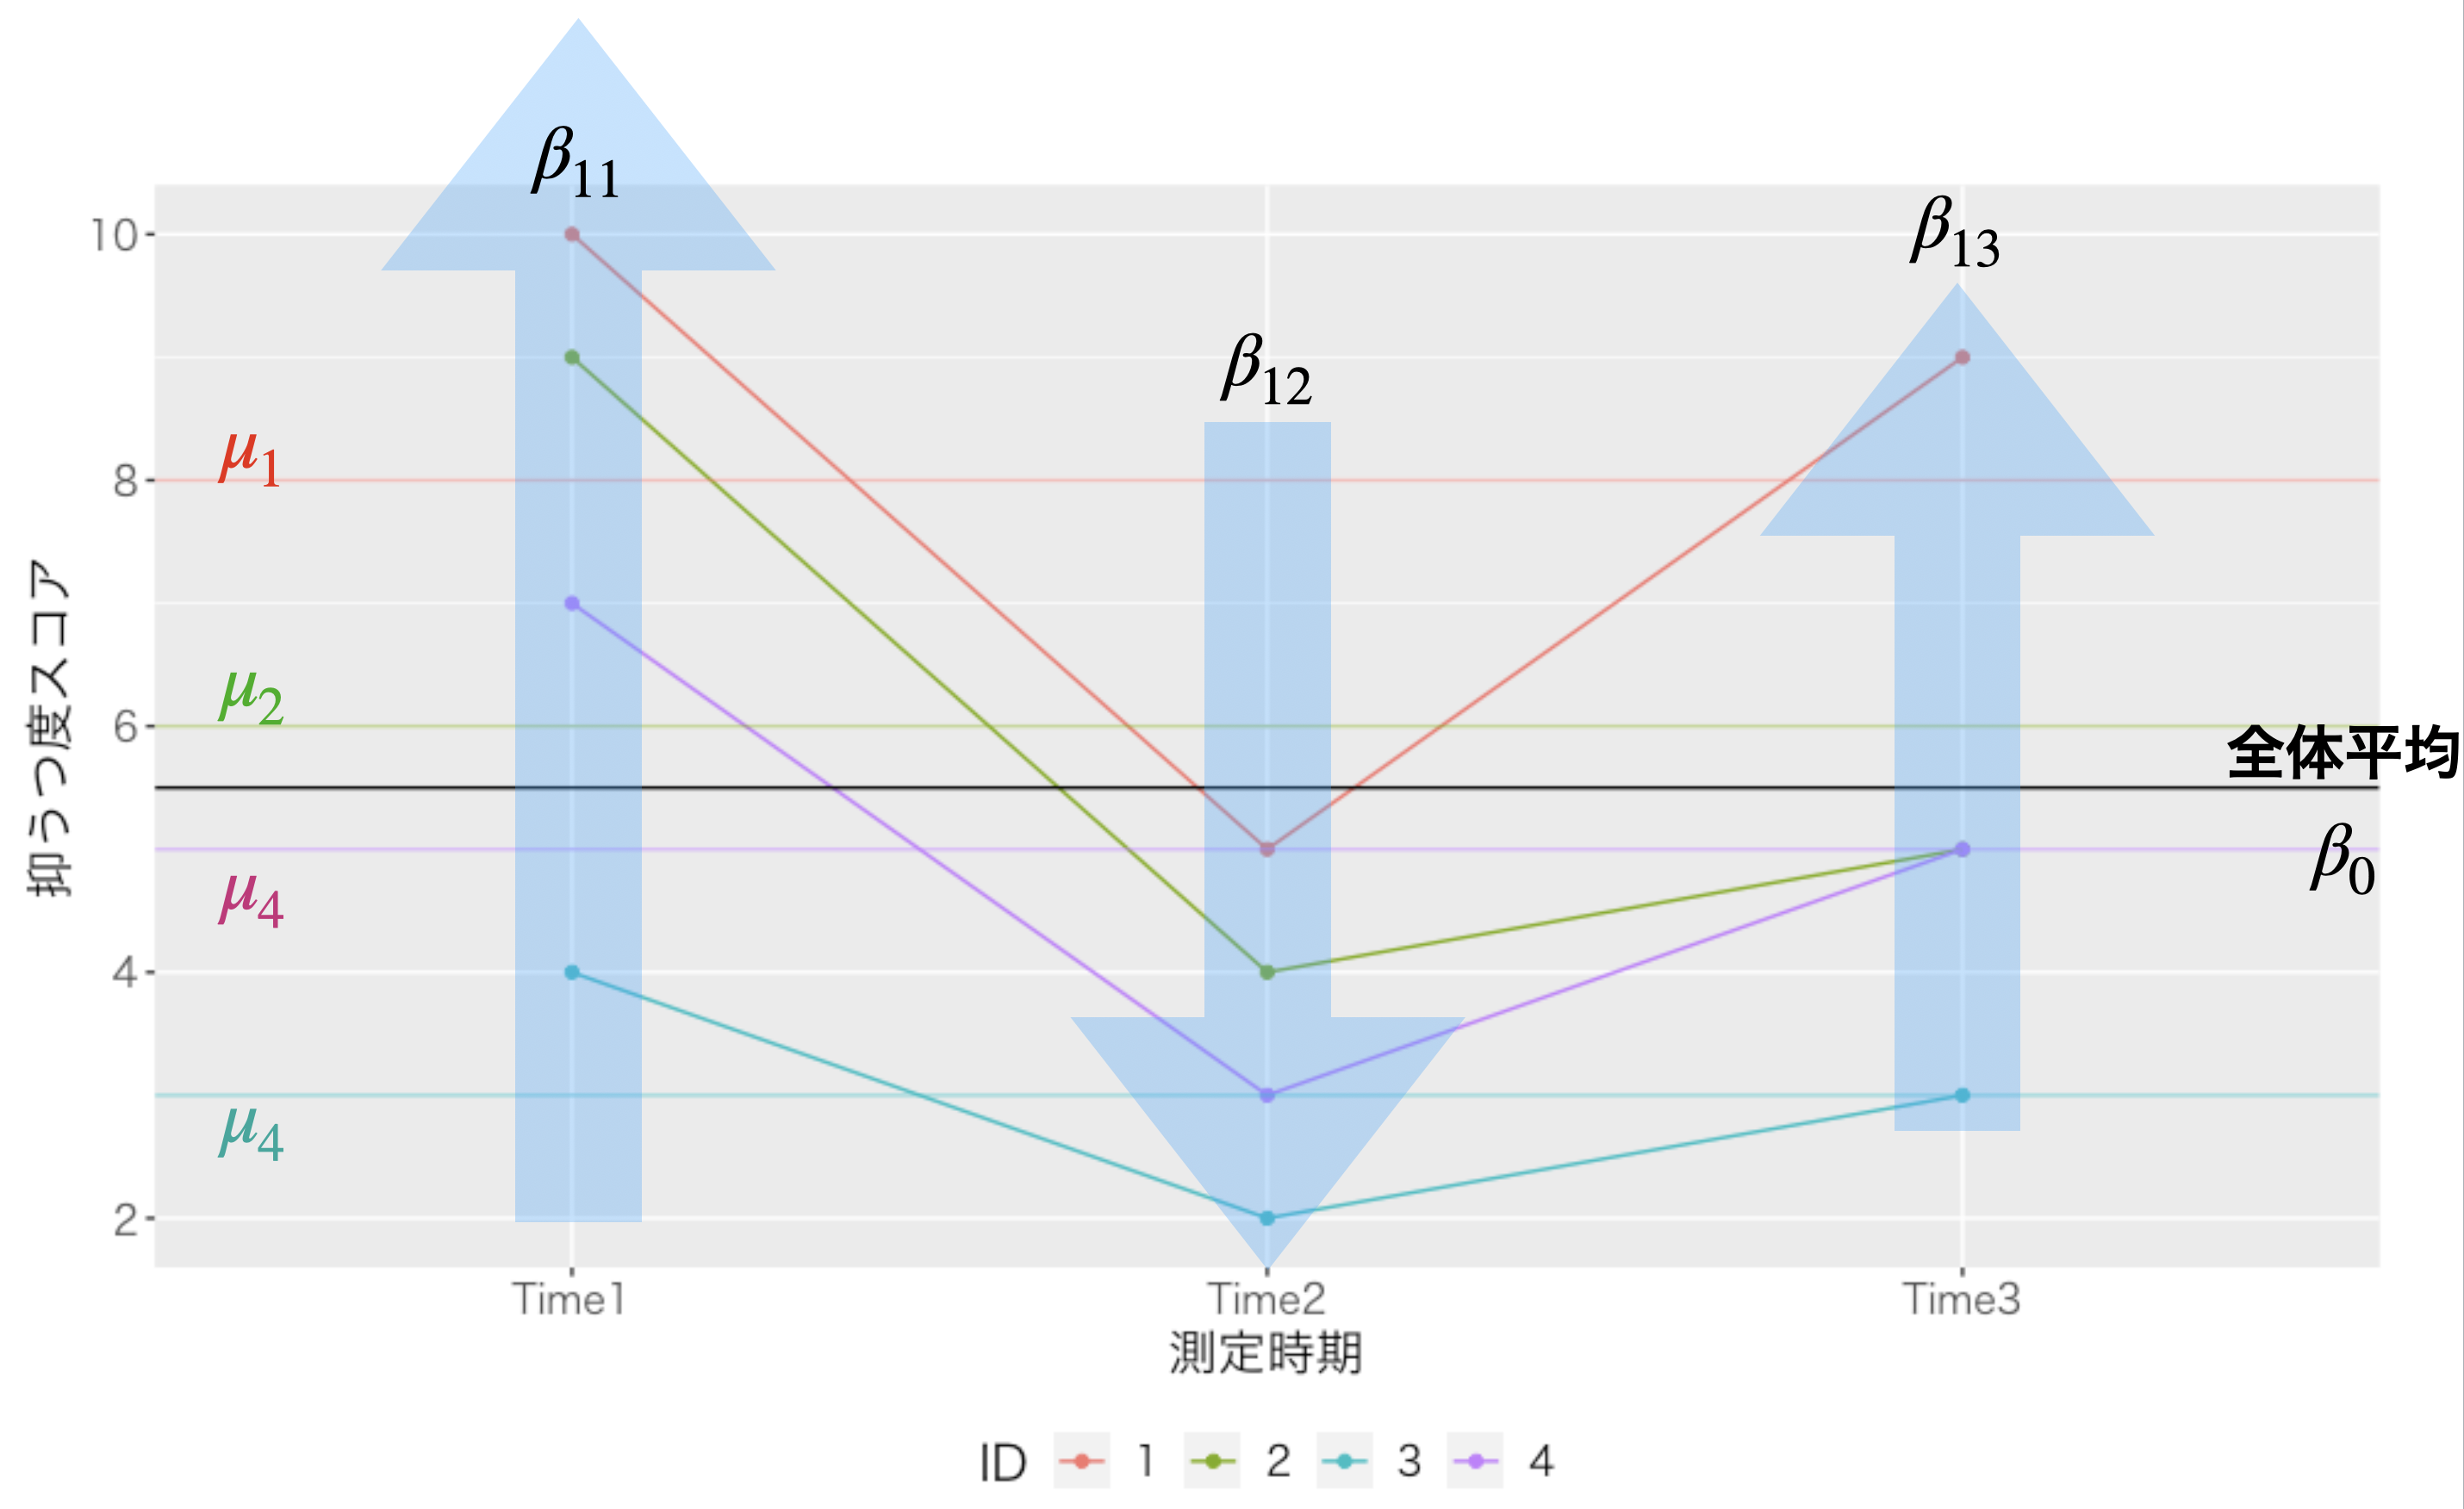
\includegraphics[keepaspectratio,width=0.8\linewidth]{../images/text22/slide22_03.png}
%   \caption{線形モデルで表現}
%   \label{fig::22_06}
% \end{figure}
% これを図で表したのが図\ref{fig::22_06}です。全体平均$\beta_0$とは別に，個別の平均$\mu_i$が計算されています。時期の効果$\beta_{1j}$は4人に等しく影響しますが，個人の平均が違うのでデータとして得られる数字はさまざまになっている，というわけです。もちろん個人差，効果を考慮しても析出できない誤差$\varepsilon_{ijk}$がありますし，これまで同様$\beta_{ij}$は相対的，つまりすべての水準を足し合わせると$0$になってしまうものです。また，個人の平均値$\mu_i$も相対的なものとして捉える必要があります。帰無仮説検定の考え方同様に，何の効果も，個人差もなかったら全体平均の横一線に並ぶはずだ，というのが基本的なアイデアだからです。

% 具体的な数字を使って考えてみましょう。表\ref{tbl::22_05}の行平均，列平均，全体平均を計算してみました。
% 行方向の平均は個人ごとの平均です。最初の人(ID=1)は平均が$8$ですから，全体平均から考えて$+2.5$の個人差がある人なのです。
% また，列方向の平均は水準ごとの平均で，これが今回みたい効果ということになります。第1期(Time1)は平均が$7.5$ですから全体平均から考えて$+2.0$の効果があった時期だ，ということです。

% 個別のデータ，たとえばID=1の第2期のデータは，理論通りに行けば，全体平均$5.5$に個人差$+2.5$と時期の効果$-2.0$が加わって出てくるはずです。$5.5+2.5-2.0＝6.0$になるはずですが，実際は$5$ですね。この違いは，理論では考えられないところなので，誤差になります。
% % latex table generated in R 4.0.2 by xtable 1.8-4 package
% % Fri Sep 11 14:57:29 2020
% \begin{table}[ht]
%   \centering
%   \caption{水準ごとの平均から効果を考える} 
%   \begin{tabular}{lrrr|r}
%     \hline
%   ID & Time1 & Time2 & Time3 & 平均\\ 
%     \hline
%   1 & 10 & 5 & 9 & 8\\ 
%     2 & 9 & 4 & 5 & 6\\ 
%     3 & 4 & 2 & 3 & 3\\ 
%     4 & 7 & 3 & 5 & 5\\ 
%      \hline
% 平均 & 7.5 & 3.5 &  5.5 &  5.5 \\\hline
%   \end{tabular}
%   \label{tbl::22_06}
%   \end{table}
% こうして，効果，個人差，誤差を計算して表にしたのが表\ref{tbl::22_07}です。平方和の計算もしてありますから，このまま分散分析に持っていけそうですね。

% % latex table generated in R 4.0.2 by xtable 1.8-4 package
% % Fri Sep 11 15:52:17 2020
% \begin{table}[ht]
%   \centering
%   \caption{効果，個人差，誤差を析出する} 
%   \begin{tabular}{llrcrrr}
%     \hline
%   ID & 時期 & スコア & 全体平均 & 個人差 & 効果 & 誤差 \\ 
%     \hline
%   1 & Time1 & 10 & 5.5 & +2.5 & +2.0 & 0.0\\ 
%     1 & Time2 & 5 & 5.5 & +2.5 & -2.0 & -1.0\\ 
%     1 & Time3 & 9 & 5.5 & +2.5 & 0.0 & +1.0\\ 
%     2 & Time1 & 9 & 5.5 & +0.5 & +2.0 & +1.0\\ 
%     2 & Time2 & 4 & 5.5 & +0.5 & -2.0 & 0.0\\ 
%     2 & Time3 & 5 & 5.5 & +0.5 & 0.0 & -1.0\\ 
%     3 & Time1 & 4 & 5.5 & -2.5 & +2.0 & -1.0\\ 
%     3 & Time2 & 2 & 5.5 & -2.5 & -2.0 & +1.0\\ 
%     3 & Time3 & 3& 5.5 & -2.5 & 0.0 & 0.0 \\ 
%     4 & Time1 & 7 & 5.5 & -0.5 & +2.0 & 0.0\\ 
%     4 & Time2 & 3 & 5.5 & -0.5 & -2.0 & 0.0\\ 
%     4 & Time3 & 5& 5.5  & -0.5 & 0.0 & 0.0 \\ 
%      \hline\hline
%   平方和&&&&39.0 & 32.0&6.0\\\hline
%   \end{tabular}
%   \label{tbl::22_07}
%   \end{table}

%   \section{帰無仮説検定としての二要因線形モデル}
%   \paragraph{仮説の設定}帰無仮説と対立仮説をたてましょう。今回も群ごとに分けた効果がない，というのが帰無仮説になります。「すべての水準における母平均に差がない」，これが帰無仮説です。対立仮説はその否定(どこかに差がある)です。
%   \paragraph{検定統計量を選択}平均値の推定ですが，今回も分散を検定対象にするので$F$分布というものを使います。
%   \paragraph{判断の基準になる確率を設定}有意水準$\alpha$，今回も5\%で勝負を決めるとしましょう。
%   \paragraph{検定統計量の実現値を計算}検定統計量$F$の実現値の計算は，先ほどの表\ref{tbl::22_06}にある平方和を基に計算します。自由度を加味して1単位あたりの効果の大きさにしてから比べますので，分散分析表にまとめて表示しちゃいましょう。

%  % latex table generated in R 4.0.2 by xtable 1.8-4 package
% % Fri Sep 11 14:39:12 2020
% \begin{table}[ht]
%   \centering
%   \caption{ANOVA Table} 
%   \begin{tabular}{lrrrrr}
%     \hline
%    & Df & SS & MS & F value & $p$ \\ 
%     \hline
%   個人差          & 3.000 & 39.000 & 13.000 &  &  \\ \hline
%     効果      & 2.000 & 32.000 & 16.000 & 16.000 & 0.0039 \\ 
%    残差\footnote{「残差」は「誤差」と同じ意味です。分散分析の文脈では，効果に入れられないもの，実験の効果を阻害するものという意味で，誤差と表現することが多いです。一方，お話ししてきたように分散分析は回帰分析(線形モデル)として考えることができますが，この場合は予測からのズレ，予測できなくて残ってしまったものという意味で，残差という言葉を使うことが多いです。同じ意味なので気にしないでください。}     & 6.000 & 6.000 & 1.000 &  &  \\ 
%      \hline
%   \end{tabular}
%     \label{tbl::22_08}
%   \end{table}
% 表\ref{tbl::22_08}には，個人差のところにラインが引いてあります。ここの$F$値は計算していません。興味がないポイントだからです。興味があるのは，あくまで「誤差に対する効果」であり，これは誤差の平均平方(MS，$6/6=1$)に対する効果の平均平方($32/2＝16$)であり，これが分子の自由度2と分母の自由度6からなるF分布の出現確率に照らし合わせて，検証することになります。

% 今回は3つの水準であり，有意であると判断できるようですから，続く検定でどこに差があったのかを掘り下げていく必要があります。この時もまた，有意水準のインフレにならないように調整が必要です。さらに効果量も併せて報告した方が良いでしょう。これらの点についても，先ほどと同じくRでの実習のところで詳しく解説します。

% \subsection{群間計画と群内計画の比較}
% 最後に，群間計画Between Designと群内計画Within Designの構造的な違いに触れておきたいと思います。

% 群内計画では，個人が誰であるかという情報があったので個人差を算出でき，それに基づいて分析しました。
% が，群内計画の時のデータを群間計画のように分析してみるとどうなるでしょうか。表\ref{tbl::22_06}にある数字が同じであれば，当然全体の平方和(分散)は同じです。ただ個人情報が抜けているのであれば，効果と誤差にしか分割できません。言い換えると，群間計画というのは誤差の中に個人差が含まれており，「これは誤差なのかな，個人差なのかな? 」という区別がつかない状態である，ということです(図\ref{fig::22_04})。

% 検定では最終的に，誤差に対する効果の大きさで検証しますから，効果が同じ＝分子が同じであれば，分母が小さい方が検定統計量$F$は大きくなり，有意であるとの判断がしやすくなります。つまり，構造的に
% \underline{群内計画の方が群間計画よりも，分析の精度が高い}ということになります。

% であれば，すべての研究が群内計画であればよいのに，と思うかもしれません。ただし，現実的な問題として，同じ人に何度も何度もデータを提供してもらうのは，非常に負担をかけることになります。研究倫理的な観点，あるいは計画上の手間を考えると，群間計画にせざるを得ないということが少なくありません。研究者，研究に協力してくれる人，のコストを考えて実験計画はデザインする必要があるということです。

% \begin{figure}[ht]
%   \centering
%   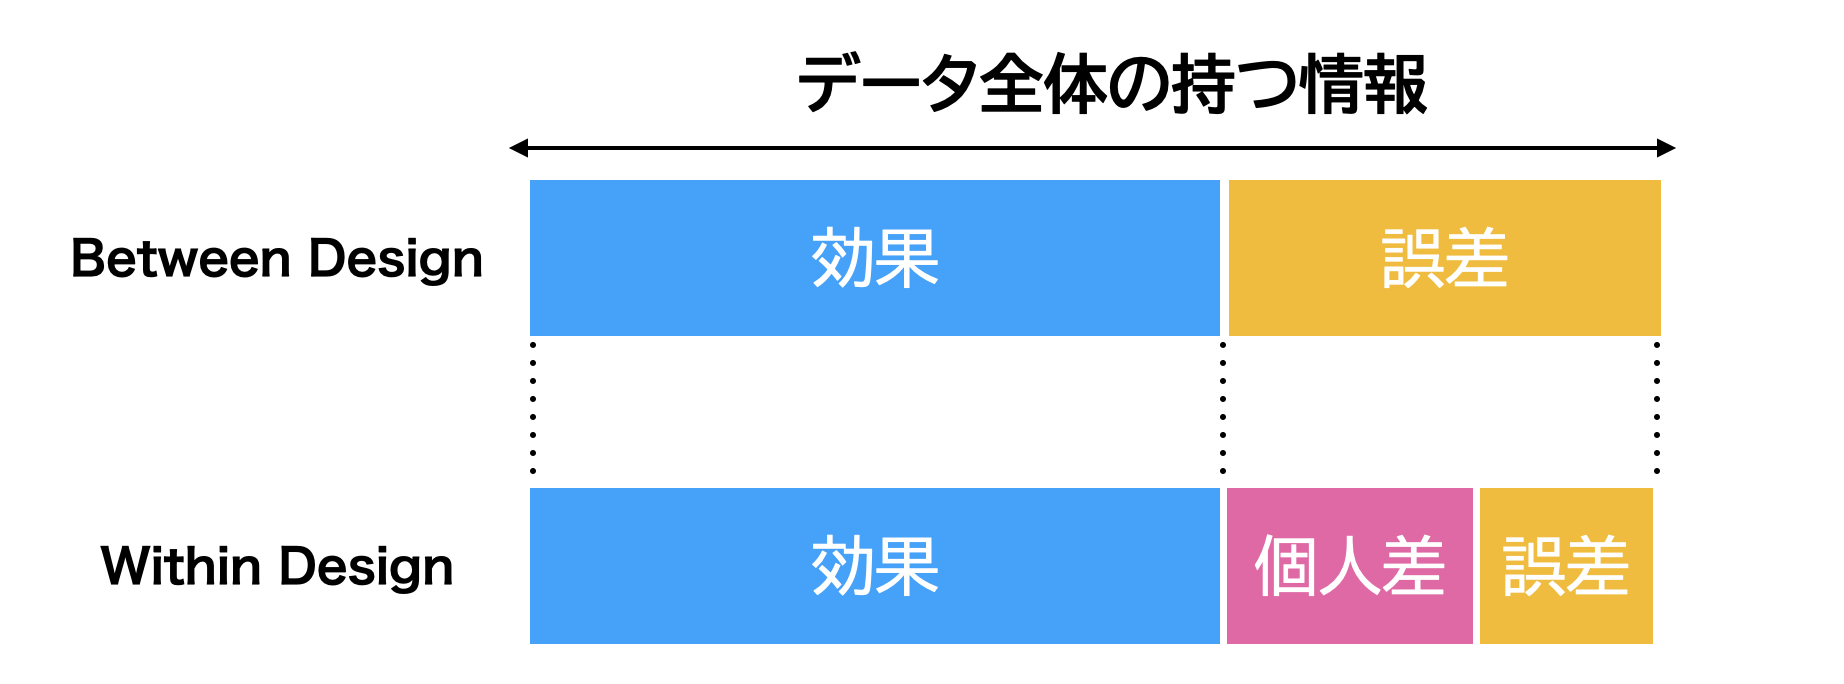
\includegraphics[keepaspectratio,width=0.8\linewidth]{../images/text22/slide22_04.png}
%   \caption{群内計画と群間計画の違い}
%   \label{fig::22_07}
% \end{figure}
%%%%%%%% 以下１３章で再利用

%また，要因が増えた時のことを思い出してください。要因の組み合わせによる影響，つまり交互作用を考えなければならない，ということがありましたね。今回は2要因の例でしたが，3要因になるとさらにその組み合わせは増えます。下に要因計画ごとの要素の組み合わせを書いてみました。
%\[
%\begin{array}{llll}
%\mbox{一要因群間計画} & \mbox{全体変動} &=& \mbox{要因A} + \mbox{誤差} \\
%\mbox{一要因群内計画} & \mbox{全体変動} &=& \mbox{要因A} + \mbox{個人差} + \mbox{誤差}\\
% \mbox{二要因群間計画} & \mbox{全体変動} &=& \mbox{要因A} + \mbox{要因B} +\mbox{交互作用AB} +\mbox{誤差}\\
% \mbox{三要因群間計画} & \mbox{全体変動} &=& \mbox{要因A} + \mbox{要因B} + \mbox{要因C}+\mbox{交互作用AB} +\mbox{交互作用AC}+\mbox{交互作用BC} \\
% &&&+\mbox{交互作用ABC}  +\mbox{誤差}\\
% \mbox{四要因群間計画} & \mbox{全体変動} &=& \mbox{要因A} + \mbox{要因B} + \mbox{要因C} + \mbox{要因D}\\
% &&&  + \mbox{交互作用AB} +\mbox{交互作用AC} +\mbox{交互作用AD}+\mbox{交互作用BC}\\
% &&& +\mbox{交互作用BD} +\mbox{交互作用CD}+\mbox{交互作用ABC}+\mbox{交互作用ABD}\\
% &&& +\mbox{交互作用BCD} +\mbox{交互作用ABCD} +\mbox{誤差}\\
%\end{array}
%\]
%3要因になると，3つの主効果(効果A,B,C)に加え，組み合わせの効果がAB,AC,BCの一次の交互作用だけでなく，ABC3つ揃った時の二次の交互作用も考える必要があります。4要因についても書いてみましたが，もう訳が分からないレベルです。

%このことからわかるように，要因計画はいくらでも複雑にしても良い，というものではありません。要因が増えるごとに考えるべき要素が増えるだけであり，結局統一的な解釈が難しくなります。お勧めとしては，交互作用のないような現象について，二要因までの研究計画にしておいた方が良いように思います。
\section{Task}

\end{document}
